\chapter{Restoring Invariants}
\label{ch:resinvs}

\newcommand{\lecnum}{18}
%\newcommand{\lectitle}{Restoring Invariants}
\newcommand{\lecturer}{Frank Pfenning}

\chapterTAGS{correctness, ds-invariant, function-pointer, pq, safety, sorting, testing}
\maketitle

\begin{preamble}
\noindent
In this lecture we will implement heaps and operations on them.  The theme of
this lecture is reasoning with invariants that are partially violated, and
making sure they are restored before the completion of an operation.  We will
only briefly review the algorithms for inserting and deleting the minimal node
of the heap; you should read the notes for the previous lecture on priority
queues and keep them close at hand.
\end{preamble}

\begin{gram}[Learning Goals]
\begin{description}
\item[Computational Thinking: ]%
  We convert ideas developed diagrammatically in the last lecture into
  working code.

\item[Algorithms and Data Structures: ]%
  Temporarily violating and restoring invariants is a common theme in
  algorithms.  It is a technique you need to master.

\item[Programming: ]%
  We practice writing generic code involving arrays.

\end{description}
\end{gram}


\section{The Heap Structure}
\label{sec:resinvs:heap_struct}
\TAGS{function-pointer, pq}

We use the following header struct to represent heaps.
\begin{lstlisting}[language={[C0]C}]
typedef struct heap_header heap;
struct heap_header {
  int limit;                      // limit = capacity+1
  int next;                       // 1 <= next && next <= limit
  elem[] data;                    // \length(data) == limit
  has_higher_priority_fn* prior;  // != NULL
};
\end{lstlisting}

\clearpage
The field \lstinline'prior' is provided by the client and tells us how to
compare elements.
\begin{lstlisting}[language={[C0]C}]
// f(x,y) returns true if e1 has STRICTLY higher priority than e2
typedef bool has_higher_priority_fn(elem e1, elem e2);
\end{lstlisting}

Since the significant array elements start at 1, as explained in the
previous lecture, the \lstinline'limit' must be one greater than the
desired capacity.  To prevent overflows, we will also require that
\lstinline'limit' be less than \lstinline'int_max()/2'.  The
\lstinline'next' index must be between \lstinline'1' and
\lstinline'limit', and the element array must have exactly
\lstinline'limit' elements.


\section{Minimal Heap Invariants}
\label{sec:resinvs:ds_invariant}
\TAGS{ds-invariant, function-pointer, pq}

Before we implement the operations, we define a function that checks
the heap invariants. The shape invariant is automatically satisfied
due to the representation of heaps as arrays, but we need to carefully
check the ordering invariants.  It is crucial that no instance of the
data structure that is not a true heap will leak across the interface
to the client, because the client may then incorrectly call operations
that require heaps with data structures that are not.

First, we check that the heap is not \lstinline'NULL', that
\lstinline'limit' has acceptable values, and that the length of the
array matches the given \lstinline'limit'.  The latter must be checked
in an annotation, because, in C0 and C1, the length of an array is not
available to us at runtime except in contracts.  Second, we check that
\lstinline'next' is in range, between $1$ and \lstinline'limit'.
Finally, we check that the client-provided comparison is defined and
non-\lstinline'NULL'.

\begin{lstlisting}[language={[C0]C}, numbers=left]
bool is_heap_safe(heap* H) {
  return H != NULL
      && (1 < H->limit && H->limit < int_max()/2)
      && is_array_expected_length(H->data, H->limit)
      && (1 <= H->next && H->next <= H->limit)
      && H->prior != NULL;
}
\end{lstlisting}
This is not sufficient to know that we have a valid heap! The
specification function \lstinline'is_heap_safe' is the minimal
specification function we need to be able to access the data
structure; we want to make sure anything we pass to the user
additionally satisfies the ordering invariant.

This invariant acts as the precondition of some of our helper
functions. We first use the client's function, accessible
as \lstinline'H->prior', to express a more useful concept for
our implementation: that the element in index \lstinline'i' can be
correctly placed as the parent of the element in index \lstinline'j' in the
heap.

\begin{lstlisting}[language={[C0]C}, numbers=left, firstnumber=9]
bool ok_above(heap* H, int i, int j)
//@requires is_heap_safe(H);
//@requires 1 <= i && i < H->next;
//@requires 1 <= j && j < H->next;
{
  return !(*H->prior)(H->data[j], H->data[i]);
}
\end{lstlisting}
This function returns \lstinline'true' whenever the element at position
\lstinline'i' has priority higher than or equal to the element at
position \lstinline'j'.

A second helper function that uses \lstinline'is_heap_safe' swaps
an element with its parent:

\begin{lstlisting}[language={[C0]C}, numbers=left, firstnumber=17]
void swap_up(heap* H, int child)
//@requires is_heap_safe(H);
//@requires 2 <= child && child < H->next;
//@requires !ok_above(H, child/2, child);  // parent == child/2
//@ensures ok_above(H, child/2, child);
{
  int parent = child/2;
  elem tmp        = H->data[child];
  H->data[child]  = H->data[parent];
  H->data[parent] = tmp;
}
\end{lstlisting}

\section{The Heap Ordering Invariant}
\label{sec:resinvs:ordering}
\TAGS{ds-invariant, pq}

It turns out to be simpler to specify the ordering invariant in the second
form seen in the last lecture, which stipulates that each node except the root
needs to be greater or equal to its parent.  To check this we iterate through
the array and compare the priority of each node \lstinline'data[i]' with its
parent, except for the root ($i = 1$) which has no parent.
\begin{lstlisting}[language={[C0]C}, numbers=left, firstnumber=29]
bool is_heap_ordered(heap* H)
//@requires is_heap_safe(H);
{
  for (int child = 2; child < H->next; child++)
  //@loop_invariant 2 <= child;
  {
    int parent = child/2;
    if (!ok_above(H, parent, child)) return false;
  }

  return true;
}

bool is_heap(heap* H) {
  return is_heap_safe(H) && is_heap_ordered(H);
}
\end{lstlisting}
Observe that the loop starts at index 2, since the root of the heap
is stored at index 1.


\section{Creating Heaps}
\label{sec:resinvs:creating}
\TAGS{correctness, pq, safety}

We start with the simple code to test if a priority queue implemented
as a heap is empty or full, and to allocate a new (empty) heap.  A
heap is empty if the next element to be inserted would be at index
$1$.  A heap is full if the next element to be inserted would be at
index \lstinline'limit' (the size of the array).
\begin{lstlisting}[language={[C0]C}, numbers=left]
bool pq_empty(heap* H)
//@requires is_heap(H);
{
  return H->next == 1;
}

bool pq_full(heap* H)
//@requires is_heap(H);
{
  return H->next == H->limit;
}
\end{lstlisting}

To create a new heap, we allocate a struct and an array
and set all the right initial values.
\begin{lstlisting}[language={[C0]C}, numbers=left, firstnumber=13]
heap* pq_new(int capacity, has_higher_priority_fn* prior)
//@requires 0 < capacity && capacity < int_max()/2 - 1;
//@requires prior != NULL;
//@ensures is_heap(\result) && pq_empty(\result);
{
  heap* H = alloc(heap);
  H->limit = capacity+1;
  H->next = 1;
  H->data = alloc_array(elem, H->limit);
  H->prior = prior;
  return H;
}
\end{lstlisting}
Note that \lstinline'H->data[0]' is unused.  We could have allocated an array
of exactly \lstinline'capacity' at the cost of complicating our index
operations.   The precondition \lstinline'capacity < int_max()/2 - 1'
wards against overflows.


\section{Insert and Sifting Up}
\label{sec:resinvs:insertion}
\TAGS{correctness, ds-invariant, pq, safety}

The shape invariant tells us exactly where to insert the new element: at the
index \lstinline'H->next' in the data array.  Then we increment the
\lstinline'next' index.
\begin{lstlisting}[language={[C0]C}, numbers=left, firstnumber=26]
void pq_add(heap* H, elem x)
//@requires is_heap(H) && !pq_full(H);
//@ensures is_heap(H);
{
  H->data[H->next] = x;
  (H->next)++;           // basic invariants hold
  // but ordering invariant may be violated
  // ...
\end{lstlisting}
By inserting $x$ in its specified place, we have, of course, violated
the ordering invariant.  We need to \emph{sift up} the new element until
we have restored the invariant.
The invariant is restored when the new element is bigger than or equal to its parent or when we have reached the root. We still need to sift up when the new element is less than its parent.
This suggests the following code:
\begin{lstlisting}[language={[C0]C}, numbers=left, firstnumber=33]
  int i = H->next - 1;      // element we just added
  while (i > 1 && !ok_above(H,i/2,i)) {
    swap_up(H, i);
    i = i/2;
  }
\end{lstlisting}
Setting \lstinline'i = i/2' is moving up in the tree, to the place we just
swapped the new element to.

At this point, as always, we should ask why accesses to the elements
of the priority queue are safe.  By short-circuiting of conjunction,
we know that $i > 1$ when we ask whether \lstinline'H->data[i/2]' is okay
above \lstinline'H->data[i]'. But we need a loop invariant to make sure
that it respects the upper bound.  The index \lstinline'i' starts at
\lstinline'H->next - 1', so it should always be strictly
less that \lstinline'H->next'.
\begin{lstlisting}[language={[C0]C}, numbers=left, firstnumber=34]
  while (i > 1 && !ok_above(H,i/2,i))
  //@loop_invariant 1 <= i && i < H->next;
  {
    swap_up(H, i);
    i = i/2;
  }
\end{lstlisting}
One small point regarding the loop invariant: we just incremented
\lstinline'H->next', so it must be strictly greater than
$1$ and therefore the invariant $1 \leq i$ must be satisfied.

But how do we know that swapping the element up the tree restores the
ordering invariant?  We need an additional loop invariant which states
that $H$ is a valid heap \emph{except at index $i$}.  Index $i$ may be
smaller than its parent, but it still needs to be less than or equal
to its children.  We therefore postulate a function
\lstinline'is_heap_except_up' and use it as a loop invariant.
\begin{lstlisting}[language={[C0]C}, numbers=left, firstnumber=34]
  while (i > 1 && !ok_above(H,i/2,i))
  //@loop_invariant 1 <= i && i < H->next;
  //@loop_invariant is_heap_except_up(H, i);
\end{lstlisting}
The next step is to write this function.  We copy the
\lstinline'is_heap_ordered' function, but check a node against its
parent only when it is different from the distinguished element where
the exception is allowed.  The differences are highlighted.
\begin{lstlisting}[language={[C0]C}]
bool is_heap_except_up(heap* H, int i) // NEW argument
//@requires is_heap_safe(H);
[*\colorbox{Yellow}{\color{\contractColor}//@\textbf{requires} 1 <= i \&\& i < H->next;}*]
{
  for (int child = 2; child < H->next; child++)
  //@loop_invariant 2 <= child;
  {
    int parent = child/2;
    if (!([*\colorbox{Yellow}{child == i ||}*]
          ok_above(H, parent, child))) return false;
  }
  return true;
}
\end{lstlisting}
We observe that \lstinline'is_heap_except_up(H, 1)' is equivalent to
\lstinline'is_heap(H)'. That's because the loop over $\mathit{child}$
starts at $2$, so the exception $\mathit{child} \not= i$ is always
true.

Now we try to prove that this is indeed a loop invariant, and therefore our
function is correct.  Rather than using a lot of text, we verify this
properties on general diagrams.  Other versions of this diagram are entirely
symmetric.  On the left is the relevant part of the heap before the swap and
on the right is the relevant part of the heap after the swap.  The relevant
nodes in the tree are labeled with their priority.  Nodes that may be above
$a$ or below $c$, $c_1$, $c_2$ and to the right of $a$ are not shown.  These
do not enter into the invariant discussion, since their relations between each
other and the shown nodes remain fixed.  Also, if $x$ is in the last row the
constraints regarding $c_1$ and $c_2$ are vacuous.
\begin{center}
  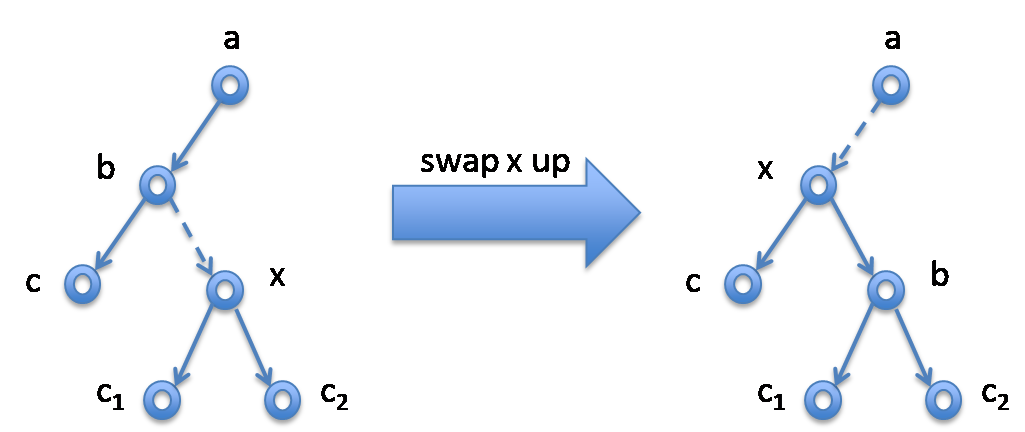
\includegraphics[width=0.9\textwidth]{img/heapup.png}
\end{center}
We know the following properties on the left from which the properties
shown on the right follow as shown:
$$
\begin{array}[t]{lll}
\text{Current iteration}
\\[1ex]
   a \leq b   & (1) & \text{order}
\\ b \leq c   & (2) & \text{order}
\\ x \leq c_1 & (3) & \text{order}
\\ x \leq c_2 & (4) & \text{order}
\\[1ex]
   b > x      & (5) & \text{since we swap}
\end{array}
\hspace{3em}
\begin{array}[t]{ll}
%\multicolumn{2}{c}{\text{\em Next iteration}}
\text{Next iteration}
\\[1ex]
   a \;?\; x  & \text{allowed exception}
\\[1ex]
   x \leq c   & \text{from $(5)$ and $(2)$}
\\ x \leq b   & \text{from $(5)$}
\\[1ex]
   b \leq c_1 & \text{??}
\\ b \leq c_2 & \text{??}
\end{array}
$$
(For this and similar examples, we'll assume that we're using a
min-heap.) Our invariant gives us no way to know that $b \leq c_1$ and
$b \leq c_2$.  We see that simply stipulating the (temporary)
invariant that every node is greater or equal to its parent except for
the one labeled $x$ is not strong enough.  It is not necessarily
preserved by a swap.

But we can strengthen it a bit.  You might want to think about
how before you move on to the next page.

\newpage
The strengthened invariant also requires that the children of the
potentially violating node $x$ are greater or equal to their
grandparent!  Let's reconsider the diagrams.
\begin{center}
  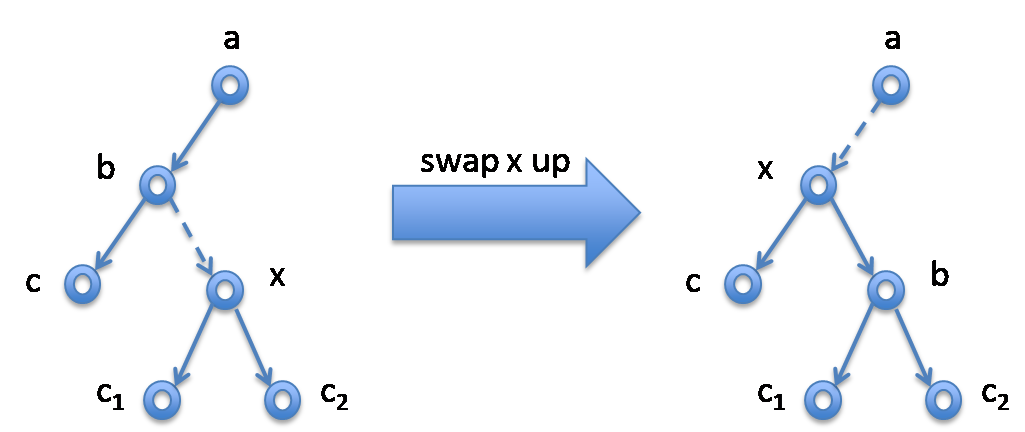
\includegraphics[width=0.9\textwidth]{img/heapup.png}
\end{center}
We have more assumptions on the left now ($(6)$ and $(7)$), but we
have also two additional proof obligations on the right ($a \leq c$
and $a \leq b$).
$$
\begin{array}[t]{lll}
%\multicolumn{3}{c}{\text{\em Current iteration}}
\text{Current iteration}
\\[1ex]
   a \leq b   & (1) & \text{order}
\\ b \leq c   & (2) & \text{order}
\\ x \leq c_1 & (3) & \text{order}
\\ x \leq c_2 & (4) & \text{order}
\\[1ex]
   b > x      & (5) & \text{since we swap}
\\[1ex]
   b \leq c_1 & (6) & \text{grandparent}
\\ b \leq c_2 & (7) & \text{grandparent}
\end{array}
\hspace{3em}
\begin{array}[t]{ll}
%\multicolumn{2}{c}{\text{\em Next iteration}}
\text{Next iteration}
\\[1ex]
   a \;?\; x  & \text{allowed exception}
\\[1ex]
   a \leq c   & \text{from $(1)$ and $(2)$}
\\ a \leq b   & \text{$(1)$}
\\[1ex]
   x \leq c   & \text{from $(5)$ and $(2)$}
\\ x \leq b   & \text{from $(5)$}
\\ b \leq c_1 & \text{$(6)$}
\\ b \leq c_2 & \text{$(7)$}
\end{array}
$$
Success!  We just need an additional function
that checks this loop invariant:

\begin{lstlisting}[language={[C0]C}]
bool grandparent_check(heap* H, int i)
//@requires is_heap_safe(H);
//@requires 1 <= i && i < H->next;
{
  int left  = 2*i;
  int right = left + 1;
  int grandparent = i/2;

  if (i == 1)          return true;        // Reached the root
  if (left >= H->next) return true;        // No children
  if (right == H->next)                    // Left child only
    return ok_above(H, grandparent, left);
  return right < H->next                   // Both children
      && ok_above(H, grandparent, left)
      && ok_above(H, grandparent, right);
}
\end{lstlisting}


Using this additional invariant, we have a loop that provably restores
the \lstinline'is_heap' invariant.

\begin{lstlisting}[language={[C0]C}, numbers=left, firstnumber=34]
  while (i > 1 && !ok_above(H,i/2,i))
  //@loop_invariant 1 <= i && i < H->next;
  //@loop_invariant is_heap_except_up (H, i);
  //@loop_invariant grandparent_check(H, i);
  {
    swap_up(H, i);
    i = i/2;
  }
\end{lstlisting}

Note that the strengthened loop invariants (or, rather, the
strengthened definition of what it means to be a heap except in one
place) is not necessary to show that the postcondition of
\lstinline'pq_add' (i.e., \lstinline'is_heap(H)') is implied.
\begin{description}
\item[Postcondition:] If the loop exits, we know the loop invariants
  and the negated loop guard are \lstinline'true':
  \begin{tabbing}
    $1 \leq i < \mathit{next}$ \` (LI 1) \\
    \lstinline'is_heap_except_up(H, i)' \` (LI 2) \\
    Either $i \leq 1$ or \lstinline'ok_above(H, i/2, i)'
    \` Negated loop guard
  \end{tabbing}
  We distinguish the two cases.
  \begin{description}
  \item[Case:] %
    \lstinline 'i <= 1'.  Then $i = 1$ from (LI 1), and
    \lstinline'is_heap_except_up(H, 1)'.  As observed before, that is
    equivalent to \lstinline'is_heap(H)'.
  \item[Case:] %
    \lstinline'ok_above(H, i/2, i)'.  Then the only possible index $i$ where
    \lstinline'is_heap_except_up(H, i)' makes an exception and does not check
    whether \lstinline'ok_above(H, i/2, i)' is actually no exception, and we
    have \lstinline'is_heap(H)'.
  \end{description}
\end{description}

\newpage
Overall, the function \lstinline'pq_add' is as follows
\begin{lstlisting}[language={[C0]C}, numbers=left, firstnumber=26]
void pq_add(heap* H, elem e)
//@requires is_heap(H) && !pq_full(H);
//@ensures is_heap(H);
{
  H->data[H->next] = e;
  (H->next)++;
  /* H may no longer be a heap! */

  int i = H->next - 1;
  while(i > 1 && !ok_above(H,i/2,i))
  //@loop_invariant 1 <= i && i < H->next;
  //@loop_invariant is_heap_except_up(H, i);
  //@loop_invariant grandparent_check(H, i);
  {
    swap_up(H, i);
    i = i/2;
  }
}
\end{lstlisting}

% Insertion is very short; we only need to make sure the heap is not
% full.  Since this is something quick to check and might be overlooked
% by the client, we use an explicit assert statement which is always
% executed, even if full dynamic checking of invariants is not enabled.
% After that, we place the new element at \lstinline'next', increment the
% \lstinline'next' index, and then call \lstinline'sift_up' in order to restore
% the invariant.
% \begin{lstlisting}[numbers=left]
% void sift_up(heap* H, int n);

% void pq_add(heap* H, int x)
% //@requires is_heap(H);
% //@ensures is_heap(H);
% {
%   assert(!pq_full(H)); /* cannot insert into full heap */
%   H->heap[H->next] = x;
%   H->next++;
%   sift_up(H, H->next-1);
% }
% \end{lstlisting}

% We now



% The difficult part is, of course, the definition of \lstinline'sift_up'.
% But we cannot write this yet, because we have no way to express
% a precondition.  Clearly, $H$ is not a valid heap, because
% the ordering invariant might be violated at $n$, the index of the new element we
% inserted.  In the left tree in the picture below, this would
% be at $n = 7$ where the new element with key $1$ is stored.
% \[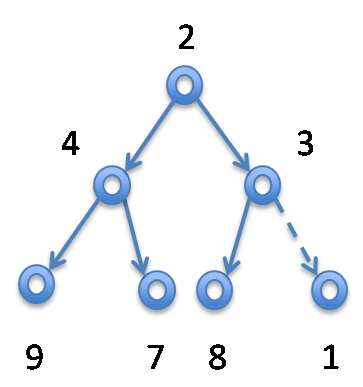
\includegraphics[width=0.99\textwidth]{img/heap3.pdf}
% \hspace*{-200pt}
% 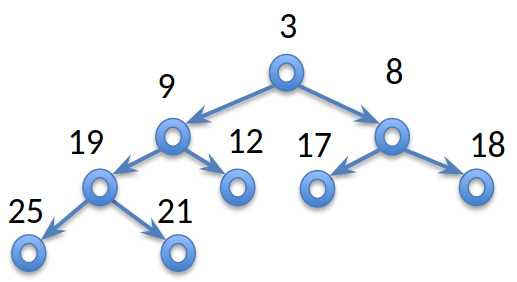
\includegraphics[width=0.99\textwidth]{img/heap4.pdf}\]
% After one step of sifting up we obtain the tree on the right,
% where the invariant is now violated at index $n = 3$.

% So we need a new function that checks if a given
% argument of type \lstinline'heap' is \emph{almost} a heap, but
% where the parent of the given node $n$ might be smaller
% than its parent.  We call this \lstinline'is_heap_except_up'.
% It is literally the same as \lstinline'is_heap', except if the
% index $i$ is equal to $n$ we do not compare with its parent.
% \begin{lstlisting}[numbers=left]
% bool is_heap_except_up(heap* H, int n) {
%   if (H == NULL) return false;
%   //@assert \length(H->heap) == H->limit;
%   if (!(1 <= H->next && H->next <= H->limit)) return false;
%   /* check parent <= node for all nodes except root (i = 1) and n */
%   for (int i = 1; i < H->next; i++)
%     //@loop_invariant 1 <= i && i <= H->next;
%     if (!(i == 1 || i == n || H->heap[i/2] <= H->heap[i])) return false;
%   return true;
% }
% \end{lstlisting}
% We can think of the crucial last test as
% \begin{lstlisting}[numbers=left]
% //@assert i == 1 || i == n || H->heap[i/2] <= H->heap[i];
% \end{lstlisting}
% rewritten as a conditional returning false.

% Now the code for \lstinline'sift_up' almost writes itself.  We start
% with a heap except at $n$ and modify it to be a true heap.
% \begin{lstlisting}[numbers=left]
% void sift_up(heap* H, int n)
% //@requires 1 <= n && n < H->limit;
% //@requires is_heap_except_up(H, n);
% //@ensures is_heap(H);
% { ... }
% \end{lstlisting}
% The body of the function consists of a loop that walks up the tree,
% swapping the new element with its parent or directly returning from the
% function if the invariant has been restored before we reach the root.
% We reach the root when the loop index $i$ has become $1$, which means
% we remain in the loop as long as $i > 1$.
% \begin{lstlisting}[numbers=left]
% void sift_up(heap* H, int n)
% //@requires 1 <= n && n < H->limit;
% //@requires is_heap_except_up(H, n);
% //@ensures is_heap(H);
% { int i = n;
%   while (i > 1)
%     //@loop_invariant is_heap_except_up(H, i);
%     {
%       if (H->heap[i/2] <= H->heap[i]) return;
%       swap(H->heap, i/2, i);  /* swap i with parent */
%       i = i/2;                /* consider parent next */
%     }
%   //@assert i == 1;
%   //@assert is_heap_except_up(H, 1);
%   return;
% }
% \end{lstlisting}
% Note how \lstinline'is_heap_except_up(H, i)' serves as a loop invariant.
% At any stage in the computation, we have a valid heap \emph{except}
% at the node we have inserted and are sifting upward in the tree.

% It is clear that if we return from the middle of the loop, then
% \lstinline'is_heap' must be satisfied, since it is satisfied everywhere
% except at $i$ (by loop invariant) and it is satisfied at $i$ when the
% condition is true.  So we can return.

% When we exit the loop and we have reached the root, we note that $H$
% is a heap except at the root.  But the root has no parent, so the heap
% invariant must be true everywhere.  Looking at the code for
% \lstinline'is_heap_except_up' we can see that the exception $i = n$
% is the same as $i = 1$ and the function behaves just like \lstinline'is_heap'.

% The postcondition is therefore established before both \lstinline'return'
% statements.

\section{Deleting the Minimum and Sifting Down}
\label{sec:resinvs:removal}
\TAGS{correctness, ds-invariant, pq, safety}

Recall that deleting the minimum swaps the root with the last element
in the current heap and then applies the \emph{sifting down} operation
to restore the invariant.  As with insert, the operation itself is
rather straightforward, although there are a few subtleties.  First,
we have to check that $H$ is a heap, and that it is not empty.  Then
we save the minimal element, swap it with the last element (at
\lstinline'next-1'), and delete the last element (now the element that
was previously at the root) from the heap by decrementing
\lstinline'next'.
\begin{lstlisting}[language={[C0]C}, numbers=left, firstnumber=80]
elem pq_rem(heap* H)
//@requires is_heap(H) && !pq_empty(H);
//@ensures is_heap(H);
{
  elem min = H->data[1];
  (H->next)--;

  if (H->next > 1) {
    H->data[1] = H->data[H->next];  // Swap last element in
    // Ordering invariant may be violated
    sift_down(H);
  }
  return min;
}
\end{lstlisting}
Next we need to restore the heap invariant by sifting down from the
root, with \lstinline'sift_down(H)'.  We only do this if there is at
least one element left in the heap.

But what is the precondition for the sifting down operation?  Again,
we cannot express this using the functions we have already written.
Instead, we need a function \lstinline'is_heap_except_down(H, i)' which
verifies that the heap invariant is satisfied in $H$, except possibly
at $i$.  This time, though, it is between $i$ and its children where
things may go wrong, rather than between $i$ and its parent as in
\lstinline'is_heap_except_up(H, i)'.  In the pictures below this would
be at $i = 1$ on the left and $i = 2$ on the right.
\begin{center}
  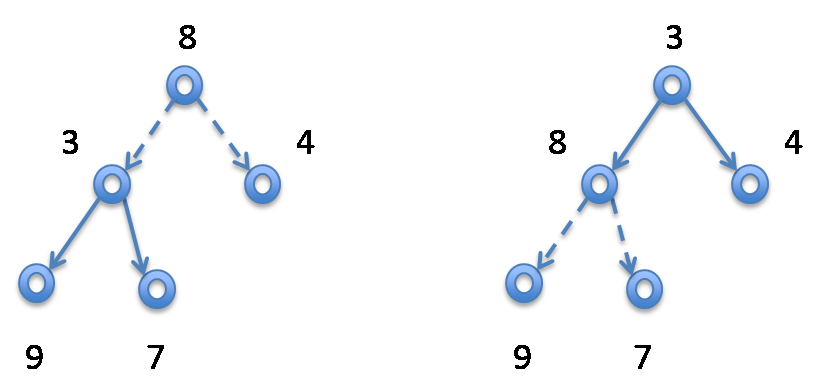
\includegraphics[width=0.7\textwidth]{img/heap7b8.png}
\end{center}
We change the test accordingly.
\begin{lstlisting}[language={[C0]C}]
/* Valid heap except at i, looking down the tree */
bool is_heap_except_down(heap* H, int i)
//@requires is_heap_safe(H);
//@requires 1 <= i && i < H->next;
{
  for (int child = 2; child < H->next; child++)
  //@loop_invariant 2 <= child;
  {
    int parent = child/2;
    if (!(parent == i || ok_above(H, parent, child))) return false;
  }
  return true;
}
\end{lstlisting}

With this we can have the right invariant to write our
\lstinline'sift_down' function.  The tricky part of this function is the
nature of the loop.  Our loop index $i$ starts at $n$ (which actually
will always be $1$ when this function is called).  We have reached
a leaf if $2i \geq \mathit{next}$ because if there is no left child,
there cannot be a right one, either.  So the outline of our function
shapes up as follows:
\begin{lstlisting}[language={[C0]C}, numbers=left, firstnumber=45]
void sift_down(heap* H)
//@requires is_heap_safe(H);
//@requires H->next > 1 && is_heap_except_down(H, 1);
//@ensures is_heap(H);
{
  int i = 1;

  while (2*i < H->next)
  //@loop_invariant 1 <= i && i < H->next;
  //@loop_invariant is_heap_except_down(H, i);
  //@loop_invariant grandparent_check(H, i);
  // ...
\end{lstlisting}
We also have written down three loop invariants: the bounds for $i$,
the heap invariant (everywhere, except possibly at $i$, looking down),
and the grandparent check, which we anticipate from our previous problems.

We want to return from the function if we have restored the invariant,
that is if the element in index $i$ is okay above all of his children.
However, there may be either 1 or 2 children (the loop guard checks that
there will be at least one).
So we have to guard this access by
a bounds check.  Clearly, when there is no right child, checking the
left one is sufficient.
\begin{lstlisting}[language={[C0]C}, numbers=left, firstnumber=52]
  while (2*i < H->next)
  //@loop_invariant 1 <= i && i < H->next;
  //@loop_invariant is_heap_except_down(H, i);
  //@loop_invariant grandparent_check(H, i);
  {
    int left = 2*i;
    int right = left+1;

    if (ok_above(H, i, left)        // All good on the left, and
        && (right >= H->next ||     // no right child or
            ok_above(H, i, right))) // all good on the right too
      return;                       // Nothing to do
    // ...
\end{lstlisting}

\clearpage
If this test fails, we have to determine the smaller of the two
children.  If there is no right child, we pick the left one, of
course.  Once we have found the smaller one we swap the current one
with the smaller one, and then make the child the new current node
$i$.

Here is the overall function:
\begin{lstlisting}[language={[C0]C}, numbers=left, firstnumber=45]
void sift_down(heap* H)
//@requires is_heap_safe(H);
//@requires H->next > 1 && is_heap_except_down(H, 1);
//@ensures is_heap(H);
{
  int i = 1;

  while (2*i < H->next)
  //@loop_invariant 1 <= i && i < H->next;
  //@loop_invariant is_heap_except_down(H, i);
  //@loop_invariant grandparent_check(H, i);
  {
    int left = 2*i;
    int right = left+1;

    if (ok_above(H, i, left)        // All good on the left, and
        && (right >= H->next ||     // no right child or
            ok_above(H, i, right))) // all good on the right too
      return;                       // Nothing to do!
    if (right >= H->next ||         // No right child, or
        ok_above(H, left, right)) { // left is smaller or equal
      swap_up(H, left);
      i = left;
    } else {                        // right is smaller
      //@assert right < H->next && ok_above(H, right, left);
      swap_up(H, right);
      i = right;
    }
  }

  //@assert i < H->next && 2*i >= H->next;
  //@assert is_heap_except_down(H, i);
  return;
}
\end{lstlisting}
Before the second return, we know that \lstinline'is_heap_except_down(H,i)'
and $2i \geq \mathit{next}$.  This means there is no node $j$ in the heap such
that $j/2 = i$ and the exception in \lstinline'is_heap_except_down' will never
apply.  $H$ is indeed a heap.

At this point we should give a proof that \lstinline'is_heap_except_down'
is really an invariant.  This is left as
Exercise~\ref{exc:sift-down-inv}.

\section{Heapsort}
\label{sec:resinvs:heapsort}
\TAGS{function-pointer, pq, sorting, testing}

We rarely discuss testing in these notes, but it is
useful to consider how to write decent test cases.  Mostly, we have
been doing random testing, which has some drawbacks but is often a
tolerable first cut at giving the code a workout.  It is \emph{much} more
effective in languages that are type safe such as C0, and even more
effective when we dynamically check invariants along the way.

In the example of heaps, one nice way to test the implementation is to
insert a random sequence of numbers, then repeatedly remove the
minimal element until the heap is empty.  If we store the elements in
an array in the order we take them out of the heap, the array should
be sorted when the heap is empty!  This is the idea behind heapsort.
We first show the code, using the random number generator we have used
for several lectures now, then analyze the complexity.  As the
priority function, we use \lstinline'int_lt(x,y)' which returns
\lstinline'true' if and only if \lstinline'x<y'.  The standard loop
invariants have been omitted for conciseness.
\begin{lstlisting}[language={[C0]C}]
int main() {
  int n = (1<<9)-1;         // 1<<9 for -d; 1<<13 for timing
  int num_tests = 10;       // 10 for -d;  100 for timing
  int seed = 0xc0c0ffee;
  rand_t gen = init_rand(seed);
  int[] A = alloc_array(int, n);
  heap* H = pq_new(n, &int_lt);

  print("Testing heap of size "); printint(n);
  print(" "); printint(num_tests); print(" times\n");
  for (int j = 0; j < num_tests; j++) {
    for (int i = 0; i < n; i++) {
      pq_add(H, rand(gen));
    }
    for (int i = 0; i < n; i++) {
      A[i] = pq_rem(H);
    }
    assert(pq_empty(H));          // heap not empty
    assert(is_sorted(A, 0, n));   // heapsort failed
  }
  print("Passed all tests!\n");
  return 0;
}
\end{lstlisting}

Now for the complexity analysis.  Inserting $n$ elements into the heap
is bounded by $O(n\log n)$, since each of the $n$ inserts is
bounded by $\log n$.  Then the $n$ element deletions are also
bounded by $O(n\log n)$, since each of the $n$ deletions is
bounded by $\log n$.  So altogether we get
$O(2n\log n) = O(n\log n)$.  Heapsort is
asymptotically as good as mergesort
or as good as the expected complexity of quicksort with random
pivots.

The sketched algorithm uses $O(n)$ auxiliary space, namely the heap.
One can use the same basic idea to do heapsort in place, using the
unused portion of the heap array to accumulate the sorted array.

Testing, including random testing, has many problems.  In our context,
one of them is that it does not test the strength of the invariants.
For example, say we write no invariants whatsoever (the weakest
possible form), then compiling with or without dynamic checking will
always yield the same test results.  We really should be testing the
invariants themselves by giving examples where they are not satisfied.
However, we should not be able to construct such instances of the data
structure on the client side of the interface.  Furthermore, within
the language we have no way to ``capture'' an exception such as a
failed assertion and continue computation.

\section{Summary}
\label{sec:resinvs:summary}
\TAGS{correctness, ds-invariant}

We briefly summarize key points of how to deal with invariants that
must be temporarily violated and then restored.
\begin{enumerate}
\item%
  Make sure you have a clear high-level understanding of why
  invariants must be temporarily violated, and how they are restored.
\item%
  Ensure that at the interface to the abstract type, only instances of
  the data structure that satisfy the full invariants are being
  passed.  Otherwise, you should rethink all the invariants.
\item%
  Write predicates that test whether the partial invariants hold for a
  data structure.  Usually, these will occur in the preconditions and
  loop invariants for the functions that restore the invariants.  This
  will force you to be completely precise about the intermediate
  states of the data structure, which should help you a lot in writing
  correct code for restoring the full invariants.
\end{enumerate}

\clearpage
\section{Exercises}
\label{sec:resinvs:exercises}

\begin{exercise}
  Write a recursive version of \lstinline'is_heap_ordered'.
\end{exercise}

\begin{exercise}
  Write a recursive version of \lstinline'is_heap_except_up'.
\end{exercise}

\begin{exercise}
  Write a recursive version of \lstinline'is_heap_except_down'.
\end{exercise}

\begin{exercise}[Sifting Down]
\label{exc:sift-down-inv}
Give a diagrammatic proof for the invariant property of sifting down
for delete (called \lstinline'is_heap_except_down'), along the lines of the
one we gave for sifting up for insert.
\end{exercise}

\begin{exercise}
  Above, we separated out the sift down operation into its own function
  \lstinline'sift_down'.  Do the same for sift up.
\end{exercise}

\begin{exercise}
  Say we want to extend priority queues so that when inserting a new
  element and the queue is full, we silently delete the element with the
  lowest priority (= maximal key value) before adding the new element.
  Describe an algorithm, analyze its asymptotic complexity, and
  provide its implementation.
\end{exercise}

\begin{exercise}
  Using the invariants described in this lecture, write a function
  \lstinline'heapsort' which sorts a given array in place by first
  constructing a heap, element by element, within the same array
  and then deconstructing the heap, element by element.

  \noindent[\textbf{Hint:} It may be easier to sort the array
  in descending order and reverse in a last pass or use
  so called max heaps where the maximal element is at the
  top.]
\end{exercise}

\begin{exercise}
  Is the array \lstinline'H->data' of a heap always sorted?
\end{exercise}

% \clearpage
% \bibliographystyle{alpha}
% \bibliography{modal}

% \cleardoublepage
